% Report describing bug in FFT based algorithm for reconstructing 2D fields
% from 1D, on-axis data.

\documentclass{report}
\usepackage{amssymb,amsmath,latexsym}
\usepackage{graphicx}
\usepackage{subfig}

\begin{document}

\title{Using FFTW to Construct 2D Fields from 1D On-Axis Data}
\maketitle

\section{Introduction}
As we all know, in OPAL, we can give it 1D on-axis field data and it can reconstruct 2D field data. For instance,
take a 1DDynamic OPAL field map. It has the following format:

\begin{equation*}
  \begin{aligned}
    &1DDynamic \quad Accuracy \\
    &zMin \quad zMax \quad numberOfZPoints \\
    &frequency \\
    &rMin \quad rMax \quad numberOfRPoints \\
    &E_{z}(n=0) \\
    &E_{z}(n=1) \\
    &. \\
    &. \\
    &. \\
    &E_{z}(n=numberOfZPoints)
  \end{aligned}
\end{equation*}
OPAL deals with this file by:
\begin{itemize}
\item Reading file data to get the field data on axis.
\item Taking FFT of data to obtain Fourier coefficients of the field.
\item Once the Fourier coefficients are calculated, OPAL can use them to calculate the field on axis and its first,
  second and third derivatives in order to find the field off axis during the actual simulation.
\end{itemize}
After checking the algorithm OPAL uses in the third step, I have concluded that it has two flaws. I have corrected the
code to reflect what I think the algorithm should be.

\section{Current Algorithm}
I will first briefly describe the algorithm OPAL uses to reconstruct the on-axis field data for a 1DDynamic field using the Fourier
coefficients from the field map data. (Other classes use the same technique.) First, the class calculates the following member
variables using the above file (I only list the ones that are important for this discussion):

\begin{enumerate}
\item $accuracy\_m = Accuracy$
\item $zbegin\_m = zMin / 100.0$ (translate from cm to m)
\item $zend\_m = zMax / 100.0$
\item $length\_m = zbegin\_m - zend\_m$
\item $num\_gridpz\_m = numberOfZPoints + 1$
\end{enumerate}
(We add 1 to numberOfZPoints so that the 1D .T7 file conforms to the same convention as is
found in the 2D Poisson/Superfish .T7 field maps.) OPAL then reads in the on axis data and uses the FFTW library to calculate
the FFT of the data to obtain the member arrays:\\ \\
$realFourCoefs\_m$ (array containing the first $accuracy\_m$ $\cos$ Fourier coefficients) \\ \\
$imagFourCoefs\_m$ (array containing the first $accuracy\_m - 1$ $\sin$ Fourier coefficients) \\
\\
Once this is done, OPAL uses the following algorithm to calculate the field on axis (which I have translated from
the code).

\begin{equation}\label{E:1}
  \begin{split}
    E_{z} &= \frac{realFourCoefs\_m[0]}{2} \\
    &+ \sum_{i=1}^{accuracy\_m - 1} \left\{realFourCoefs\_m[i] * \cos \left(2 \pi i \frac{z - zbegin\_m}{length\_m}\right) \right.\\
    &\phantom{+ \sum_{i=1}^{accuracy\_m - 1} \left\{\right.}
    \left. + imagFourCoeffs\_m[i] * \sin \left(2 \pi i \frac{z - zbegin\_m}{length\_m}\right) \right\}
  \end{split}
\end{equation}

\section {New Algorithm}
I claim that \eqref{E:1} has two errors. The correct equation should be:

\begin{equation}\label{E:2}
  \begin{split}
    &E_{z} = \frac{realFourCoefs\_m[0]}{2} \\
    &+ \sum_{i=1}^{accuracy\_m - 1} \left\{realFourCoefs\_m[i] * \cos \left(2 \pi i \frac{z - zbegin\_m}{length\_m
          + \Delta z}\right) \right.\\
    &\phantom{+ \sum_{i=1}^{accuracy\_m - 1} \left\{\right.}
    \left. - imagFourCoeffs\_m[i] * \sin \left(2 \pi i \frac{z - zbegin\_m}{length\_m + \Delta z}\right) \right\}
  \end{split}
\end{equation}
where the new term $\Delta z$ is given by:

\begin{equation*}
  \Delta z \equiv \frac{length\_m}{num\_gridpz\_m - 1}
\end{equation*}
The two differences is the addition of $\Delta z$ and the change in sign in front of $imagFourCoeffs\_m[i]$.

To test these two algorithms, I added a few lines to OPAL so that, when first called, the 1DDynamic class would calculate the
field on axis, write it to file and then exit. I then changed the code to use \eqref{E:2} instead of \eqref{E:1}. I then tested
the two algorithms against each other using three different 1D field maps:

\begin{itemize}
\item CTF3.T7 - This is the field map of the CTF3 photoinjector.
\item FINSB-RAC.T7 - This is the field map used for the PSI-XFEL injector s-band travelling wave structures.
\item FINLB01-MSLAC-1D.T7 - This is a field map derived from a solenoid map used in the PSI-XFEL. This field was used because
  it is a sin like function, unlike the first two that are cos like.
\end{itemize}

The results of the three tests are shown in Figures~\ref{Fi:figure-1}, \ref{Fi:figure-2} and \ref{Fi:figure-3}. Each figure
contains three plots. The first is of the field itself showing the original data, the field as reconstructed by the original
algorithm \eqref{E:1} and the field reconstructed by the new algorithm \eqref{E:2}. The next two plots show the differences
between the original data and the reconstructed fields. In every case, I used a value of 40 for $accuracy\_m$. The new
algorithm gives much better results.

\section{Why the Changes?}
According to the FFTW website, the FFTW library calculates the transform:

\begin{equation}\label{E:3}
  Y_{k} = \sum_{j = 0}^{n - 1}X_{j}e^{\frac{-2 \pi j k \sqrt{-1}}{n}}
\end{equation}
where $Y_{k}$ are the complex FFT coefficients. These coefficients are unnormalized, so must be divided by $n$ before OPAL
can use them. So, the coefficients $a_{k}$ and $b_{k}$ from the cos/sin series formulation (which is what OPAL uses) are related
to $Y_{k}$ by:

\begin{equation*}
  \begin {aligned}
    a_{0} = \frac{Re\left(Y_{0}\right)}{n} \\
    a_{k \ne 0} = 2 \frac{Re\left(Y_{k}\right)}{n} \\
    b_{k} = - 2 \frac{Re\left(Y_{k}\right)}{n}
  \end{aligned}
\end{equation*}
In OPAL, we are missing the minus sign for $b_{k}$.

The other change in \eqref{E:2} versus \eqref{E:1} is the addition of $\Delta z$ to $length\_m$. This comes about because
in our field map the field starts at $z = zbegin\_m$ when our index in the sum in \eqref{E:3} is $j = 0$. When $j = n - 1$, the
last term in the sum, our field is at $z = zend\_m$. In \eqref{E:3}, the exponent term is divided by $n$. However, in \eqref{E:1}
we divide by $length\_m = zend\_m - zbegin\_m$ in the cos and sin terms, which is equivalent to $n - 1 - 0 = n - 1$. Therefore,
to get the correct normalization, we need to add one more ``increment'' ($\Delta z$) to $length\_m$ to get the correct
formula (as shown in \eqref{E:2}).

\begin{figure}[hbt]
  \centering
  \subfloat[][]{
    \label{Fi:figure-1a}
    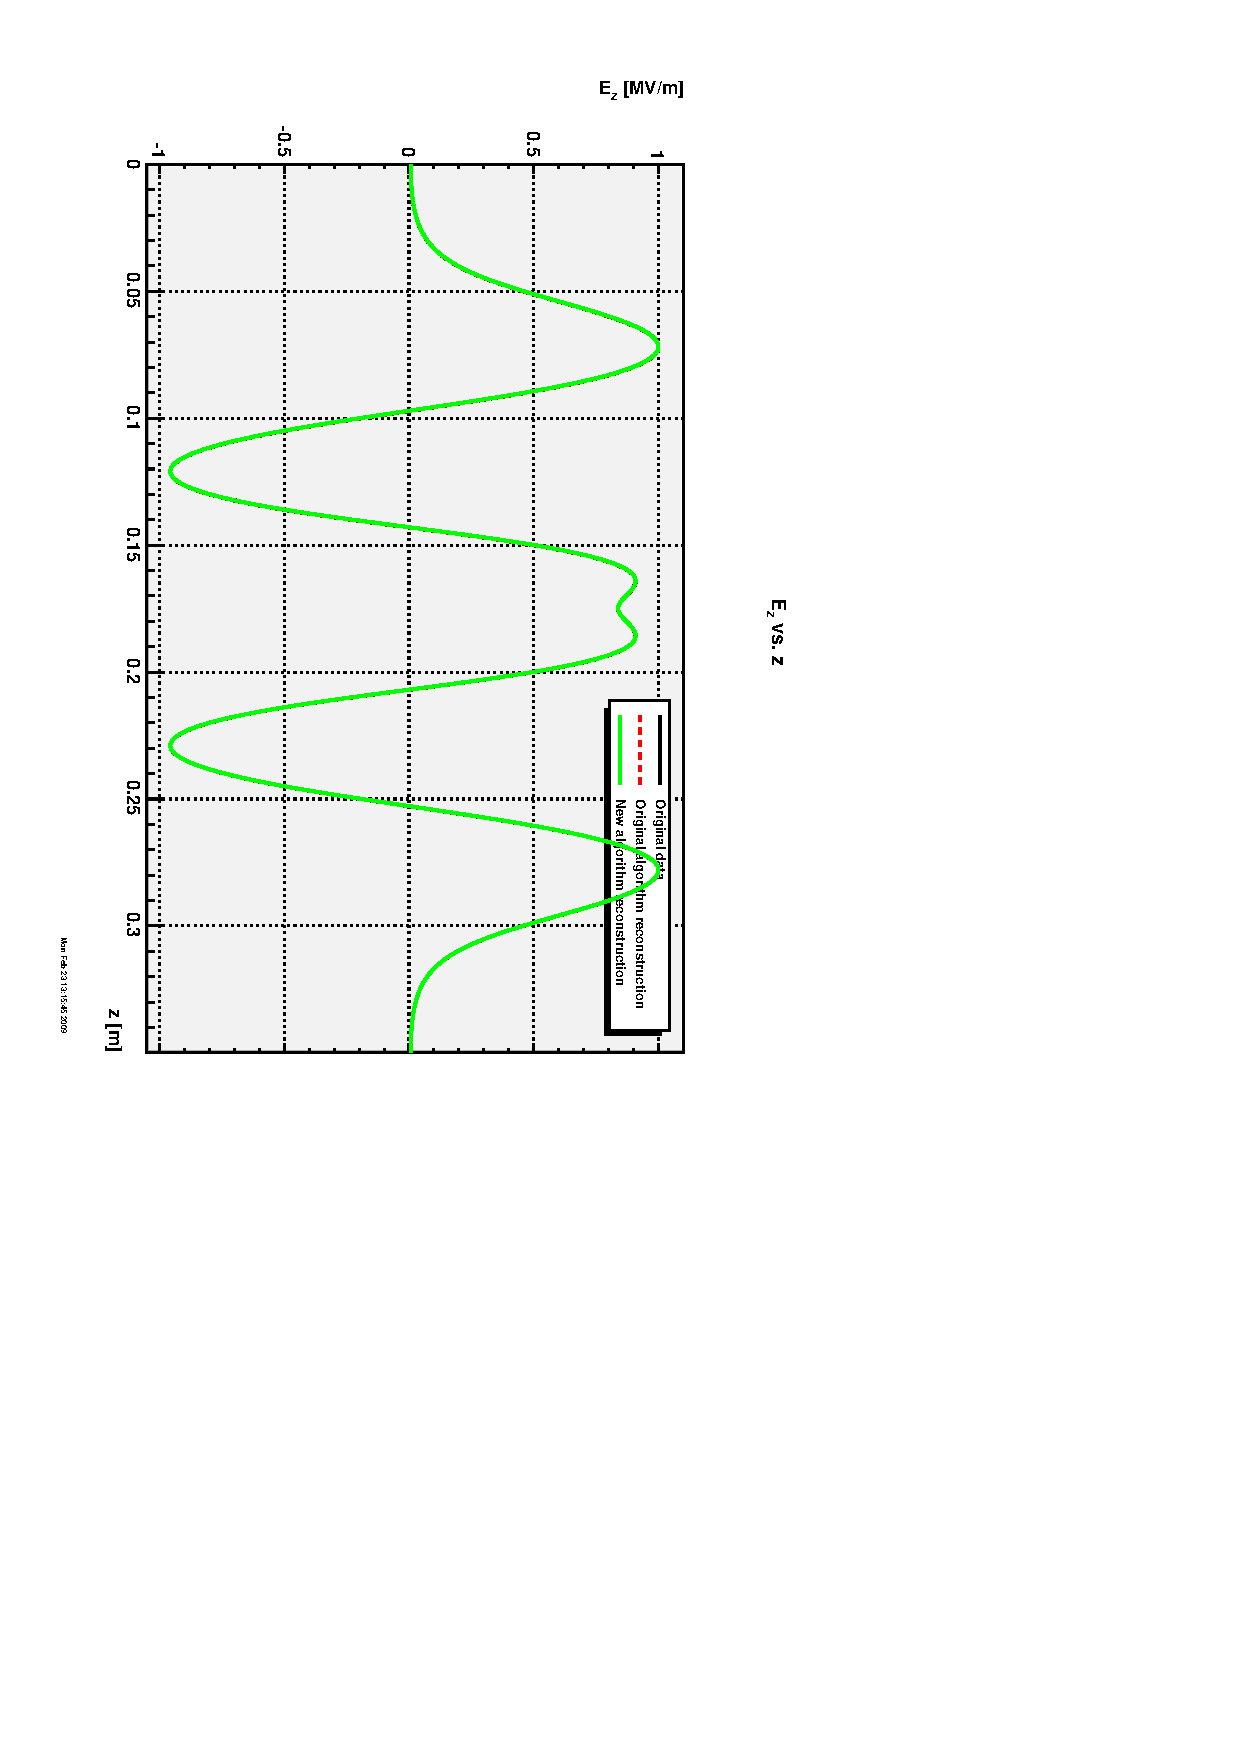
\includegraphics[scale=0.4,angle=90.0]{field-CTF3.pdf}} \\
  \subfloat[][]{
    \label{Fi:figure-1b}
    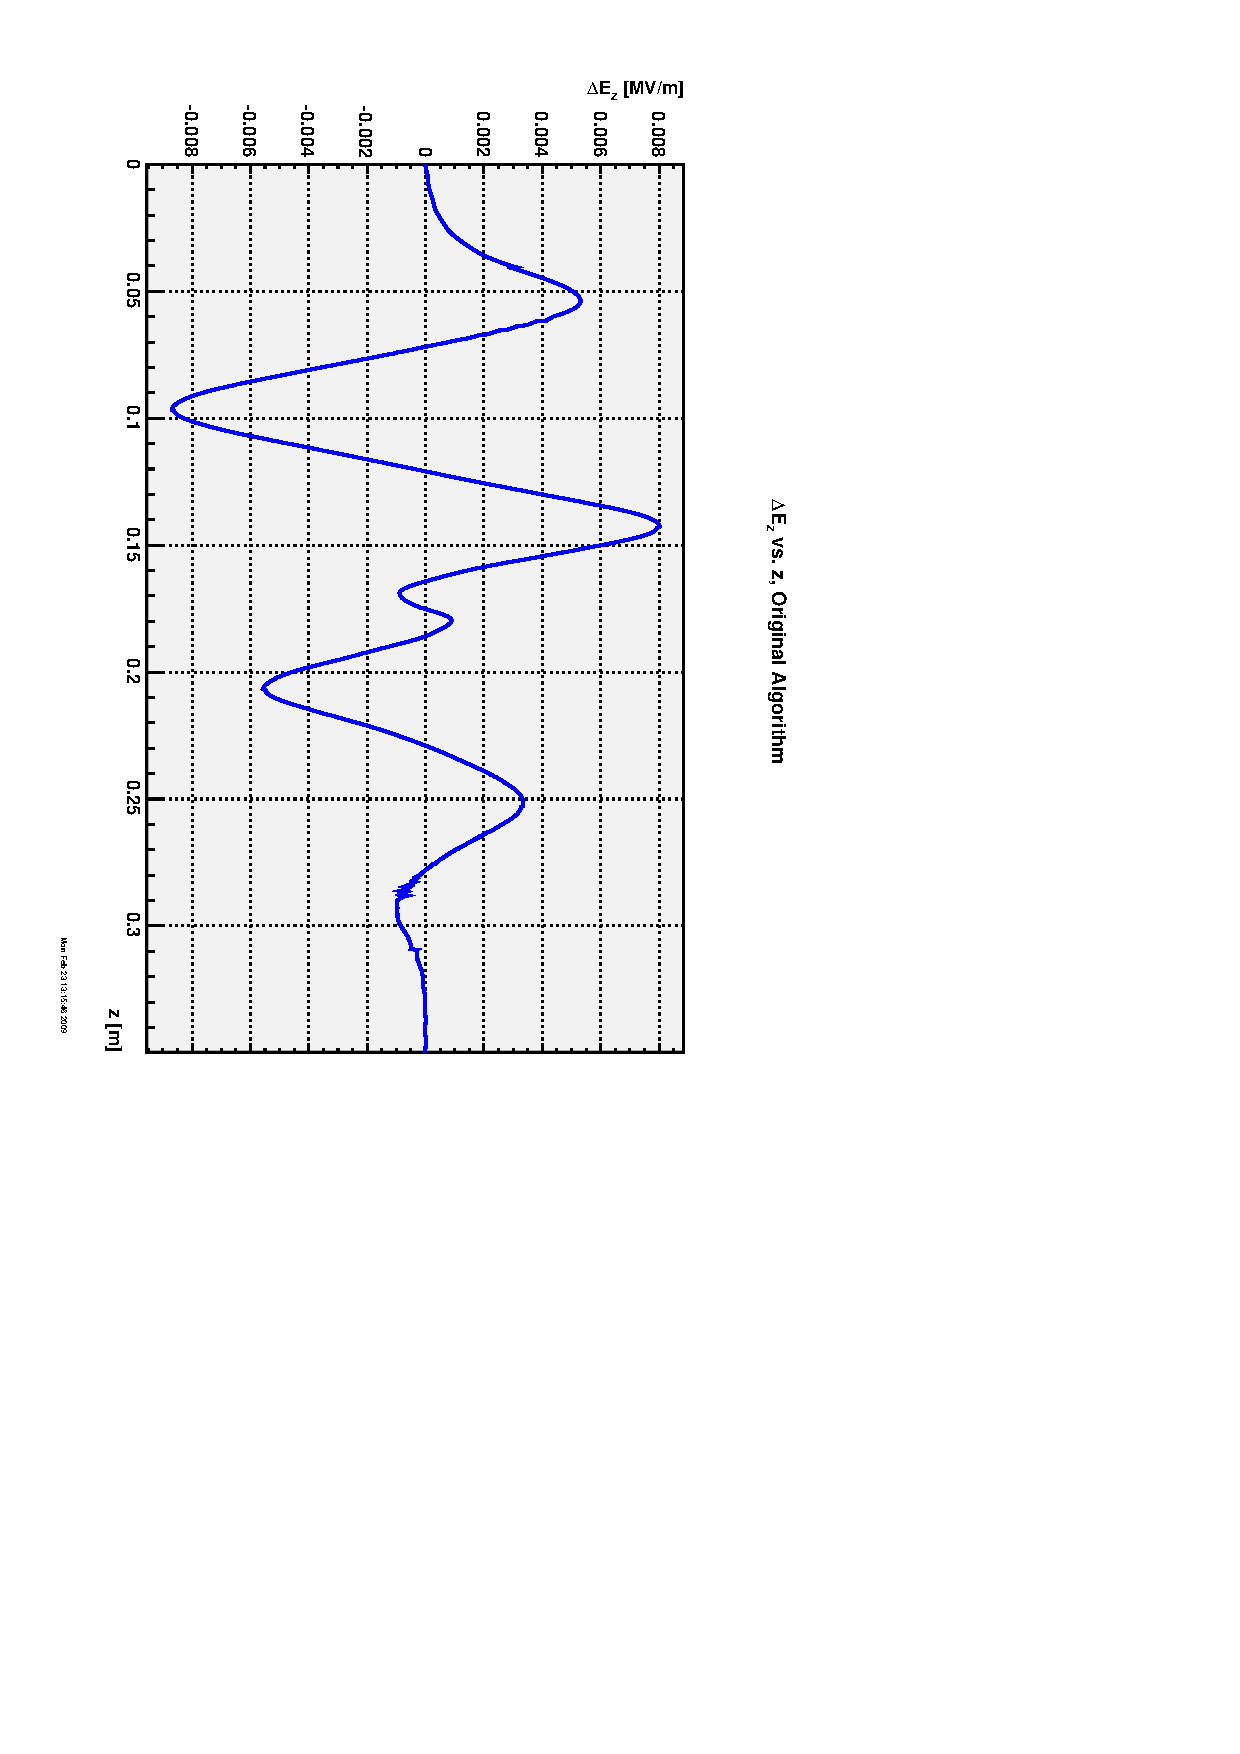
\includegraphics[scale=0.4,angle=90.0]{field-diff-original-CTF3.pdf}} \\
  \subfloat[][]{
    \label{Fi:figure-1c}
    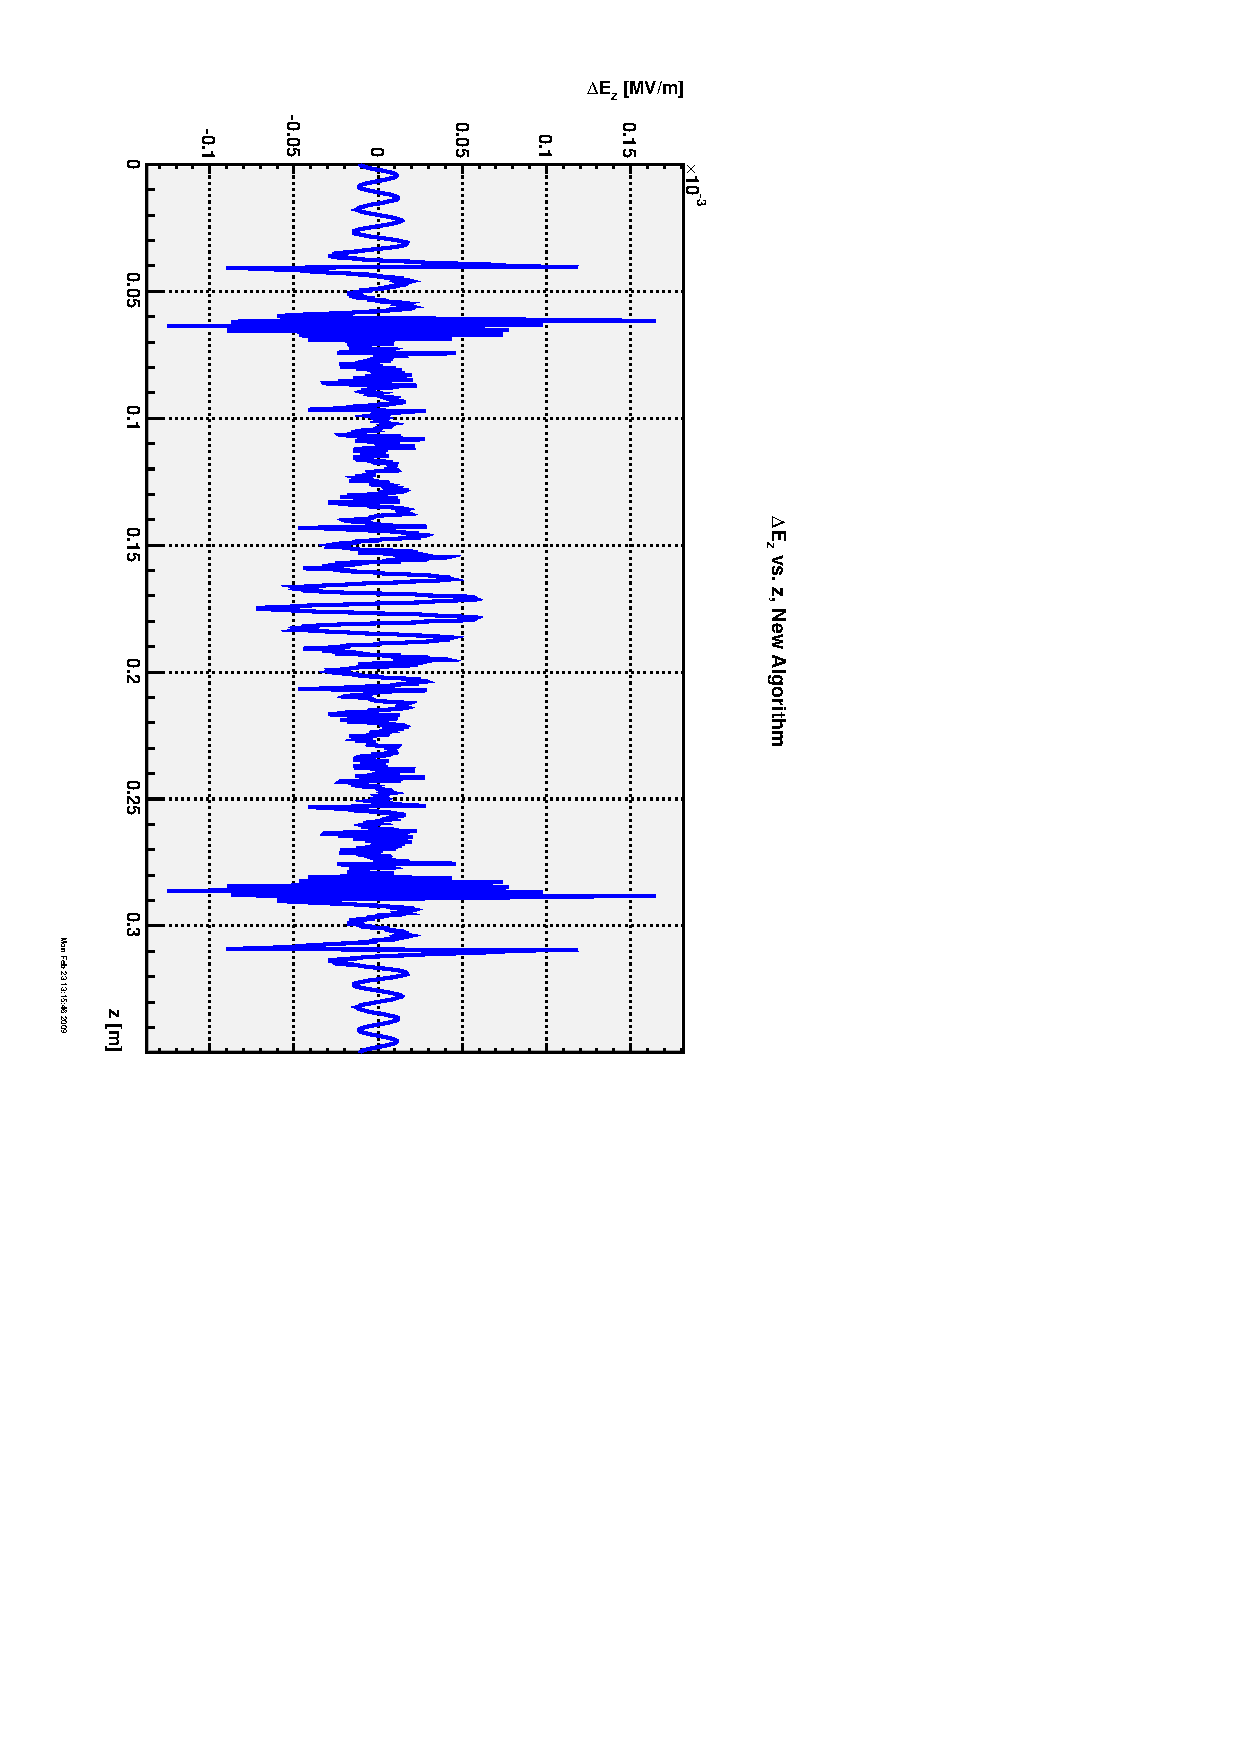
\includegraphics[scale=0.4,angle=90.0]{field-diff-new-CTF3.pdf}}
  \caption{Comparison of reconstruction algorithms \eqref{E:1} and \eqref{E:2} using CTF3.T7 field file. \subref{Fi:figure-1a}
    Field from data, reconstruction using \eqref{E:1} (original) and reconstruction using \eqref{E:2} (new).
    \subref{Fi:figure-1b} Difference between original field and field reconstructed using \eqref{E:1}. \subref{Fi:figure-1c}
    Difference between original field and field reconstructed using \eqref{E:2}.}
  \label{Fi:figure-1}
\end{figure}

\begin{figure}[hbt]
  \centering
  \subfloat[][]{
    \label{Fi:figure-2a}
    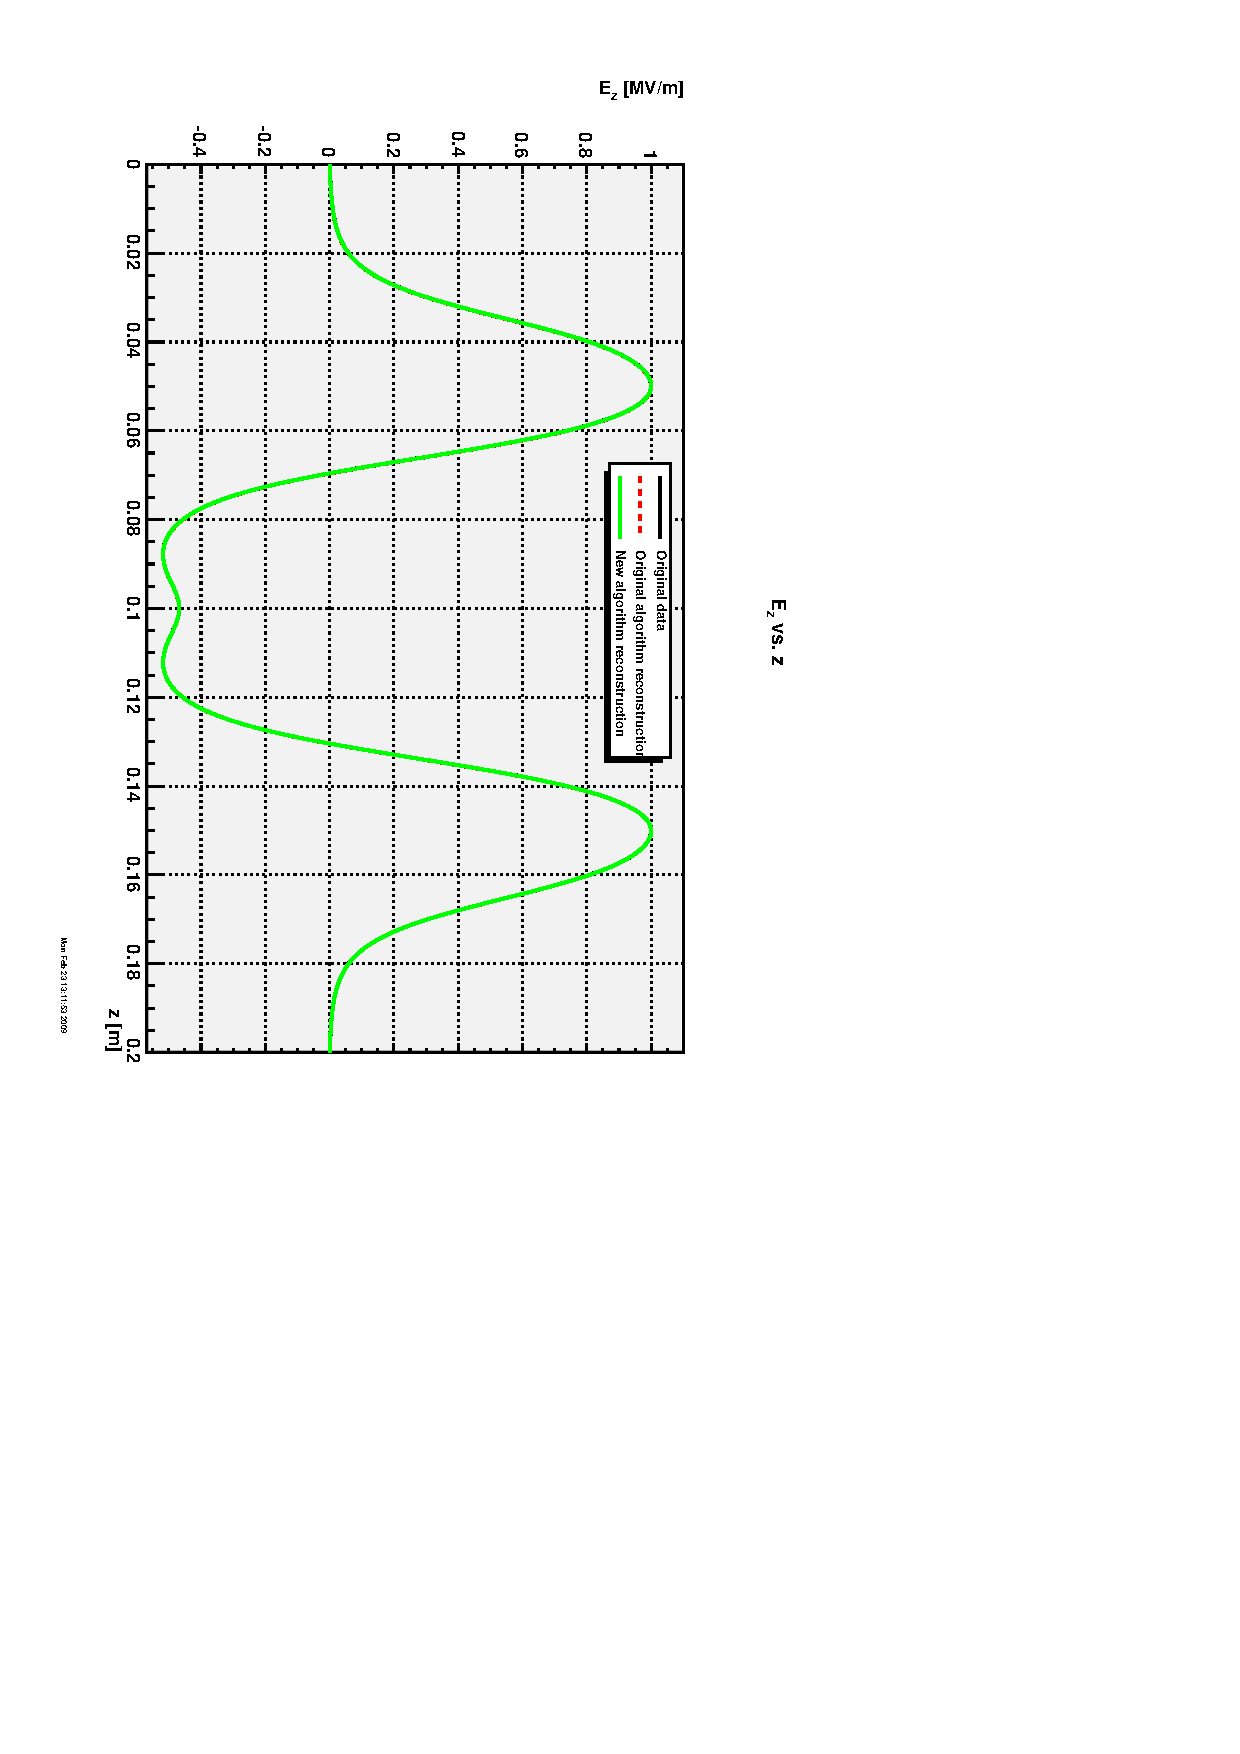
\includegraphics[scale=0.4,angle=90.0]{field-FINSB-RAC.pdf}} \\
  \subfloat[][]{
    \label{Fi:figure-2b}
    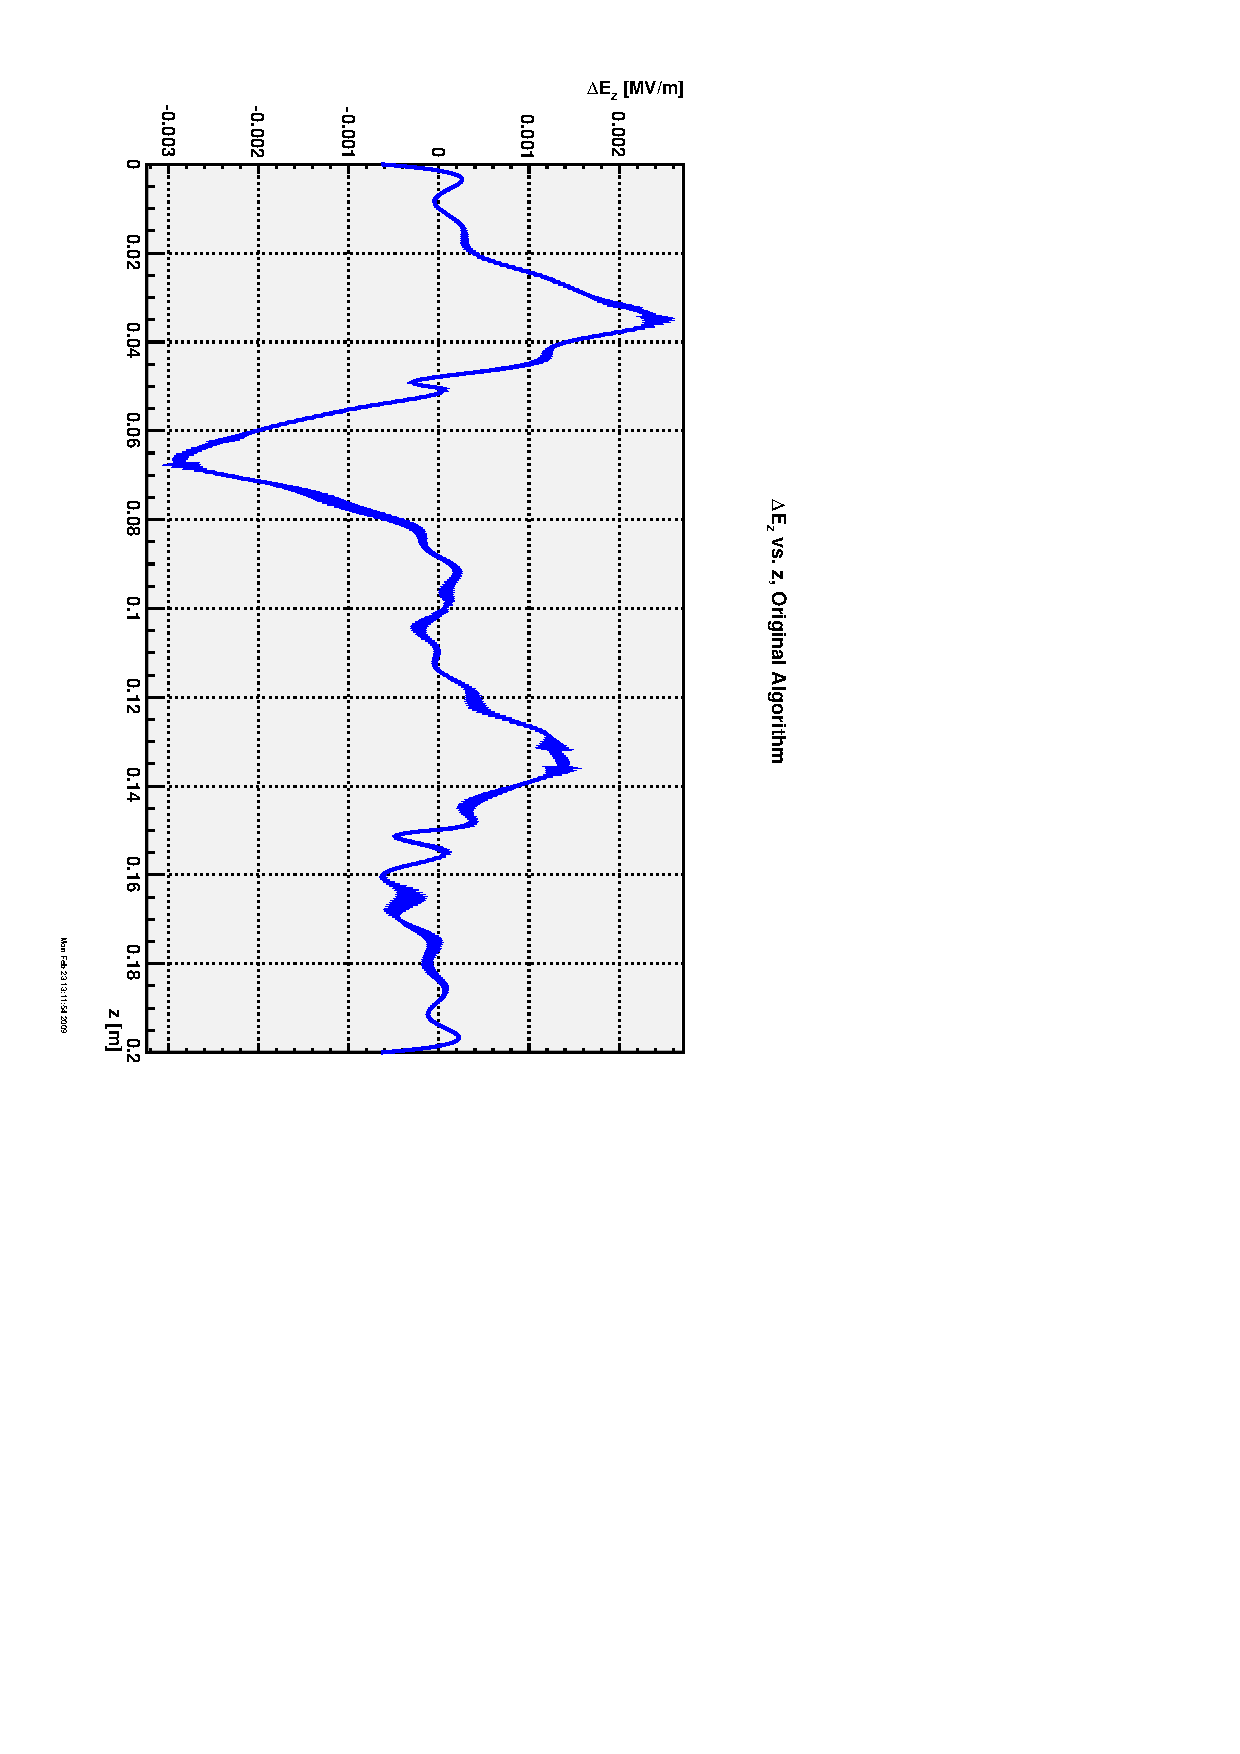
\includegraphics[scale=0.4,angle=90.0]{field-diff-original-FINSB-RAC.pdf}} \\
  \subfloat[][]{
    \label{Fi:figure-2c}
    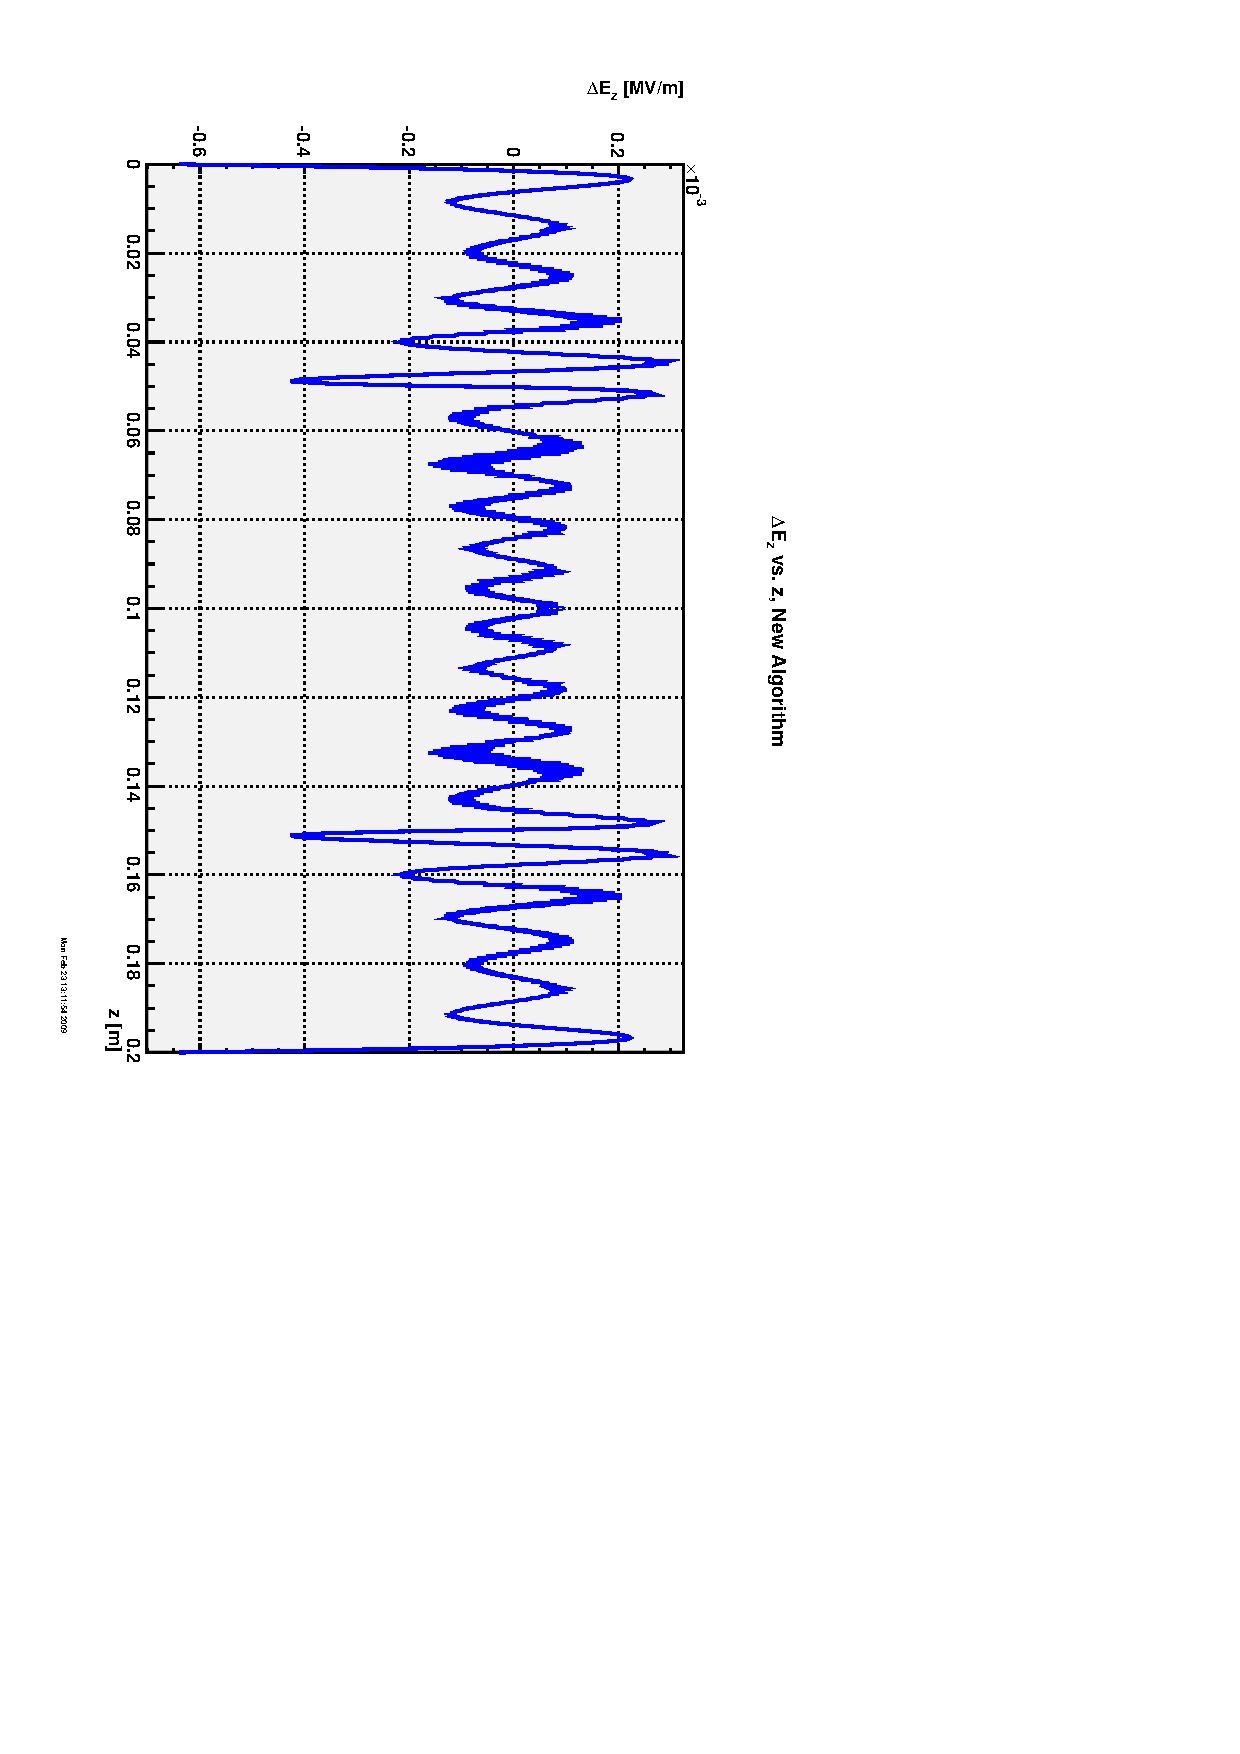
\includegraphics[scale=0.4,angle=90.0]{field-diff-new-FINSB-RAC.pdf}}
  \caption{Comparison of reconstruction algorithms \eqref{E:1} and \eqref{E:2} using FINSB-RAC.T7 field file.
    \subref{Fi:figure-2a} Field from data, reconstruction using \eqref{E:1} (original) and reconstruction using
    \eqref{E:2} (new). \subref{Fi:figure-2b} Difference between original field and field reconstructed using \eqref{E:1}.
    \subref{Fi:figure-2c} Difference between original field and field reconstructed using \eqref{E:2}.}
  \label{Fi:figure-2}
\end{figure}

\begin{figure}[hbt]
  \centering
  \subfloat[][]{
    \label{Fi:figure-3a}
    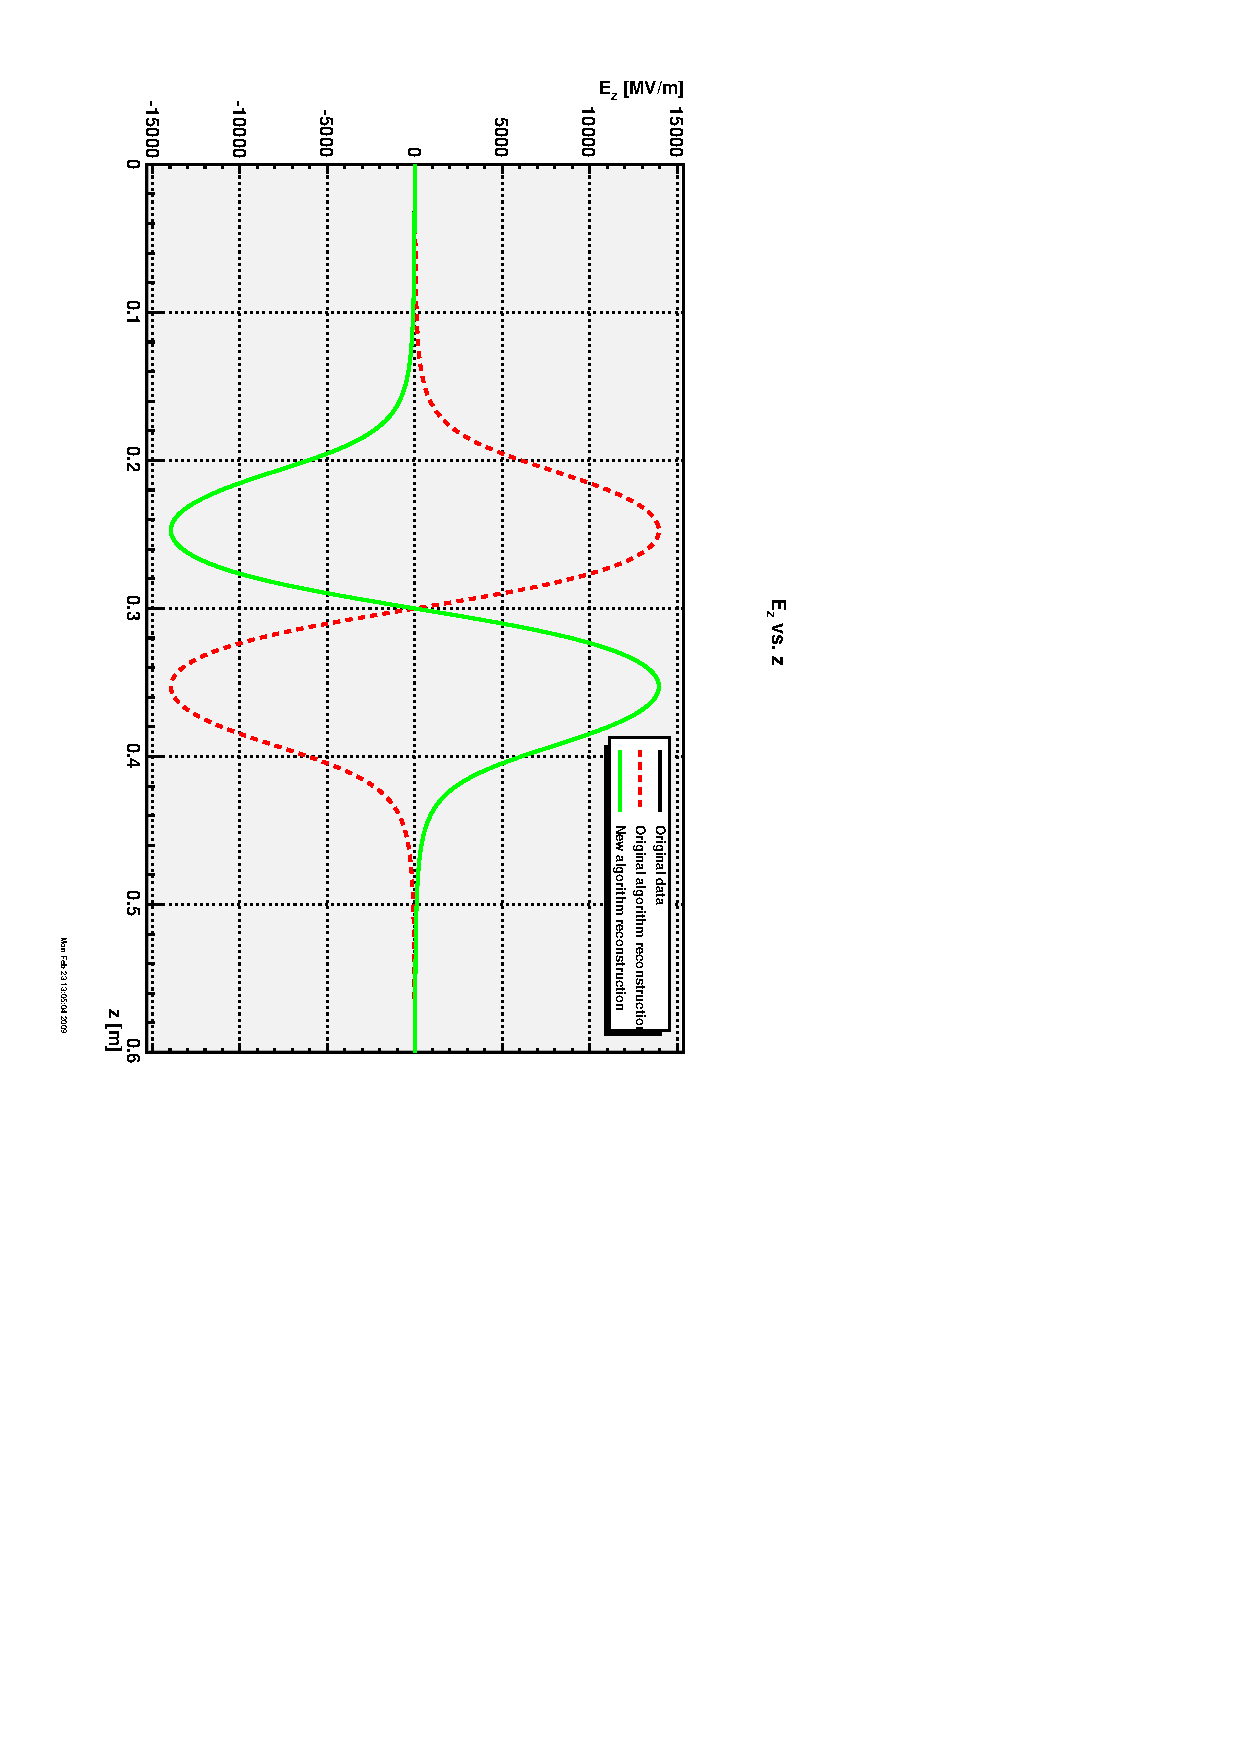
\includegraphics[scale=0.4,angle=90.0]{field-FINLB01-MSLAC.pdf}} \\
  \subfloat[][]{
    \label{Fi:figure-3b}
    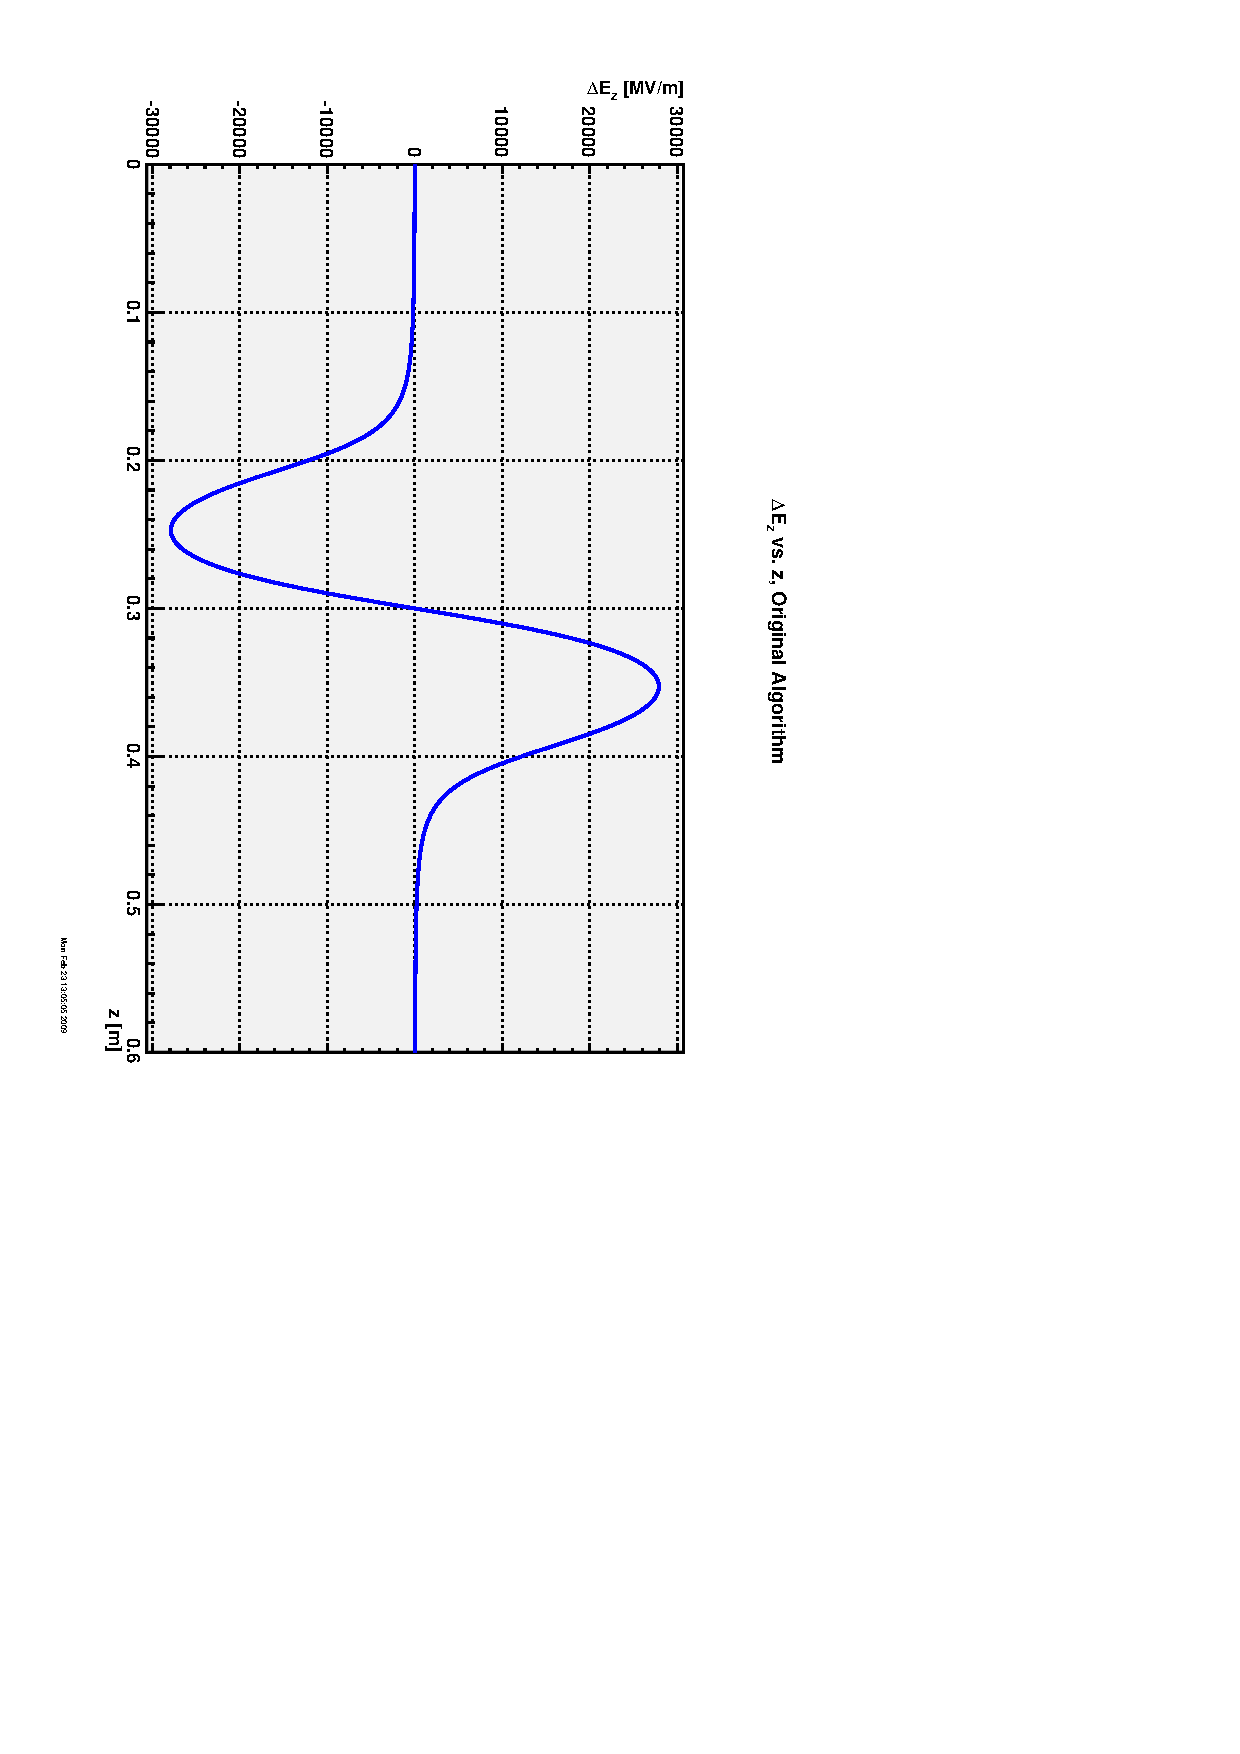
\includegraphics[scale=0.4,angle=90.0]{field-diff-original-FINLB01-MSLAC.pdf}} \\
  \subfloat[][]{
    \label{Fi:figure-3c}
    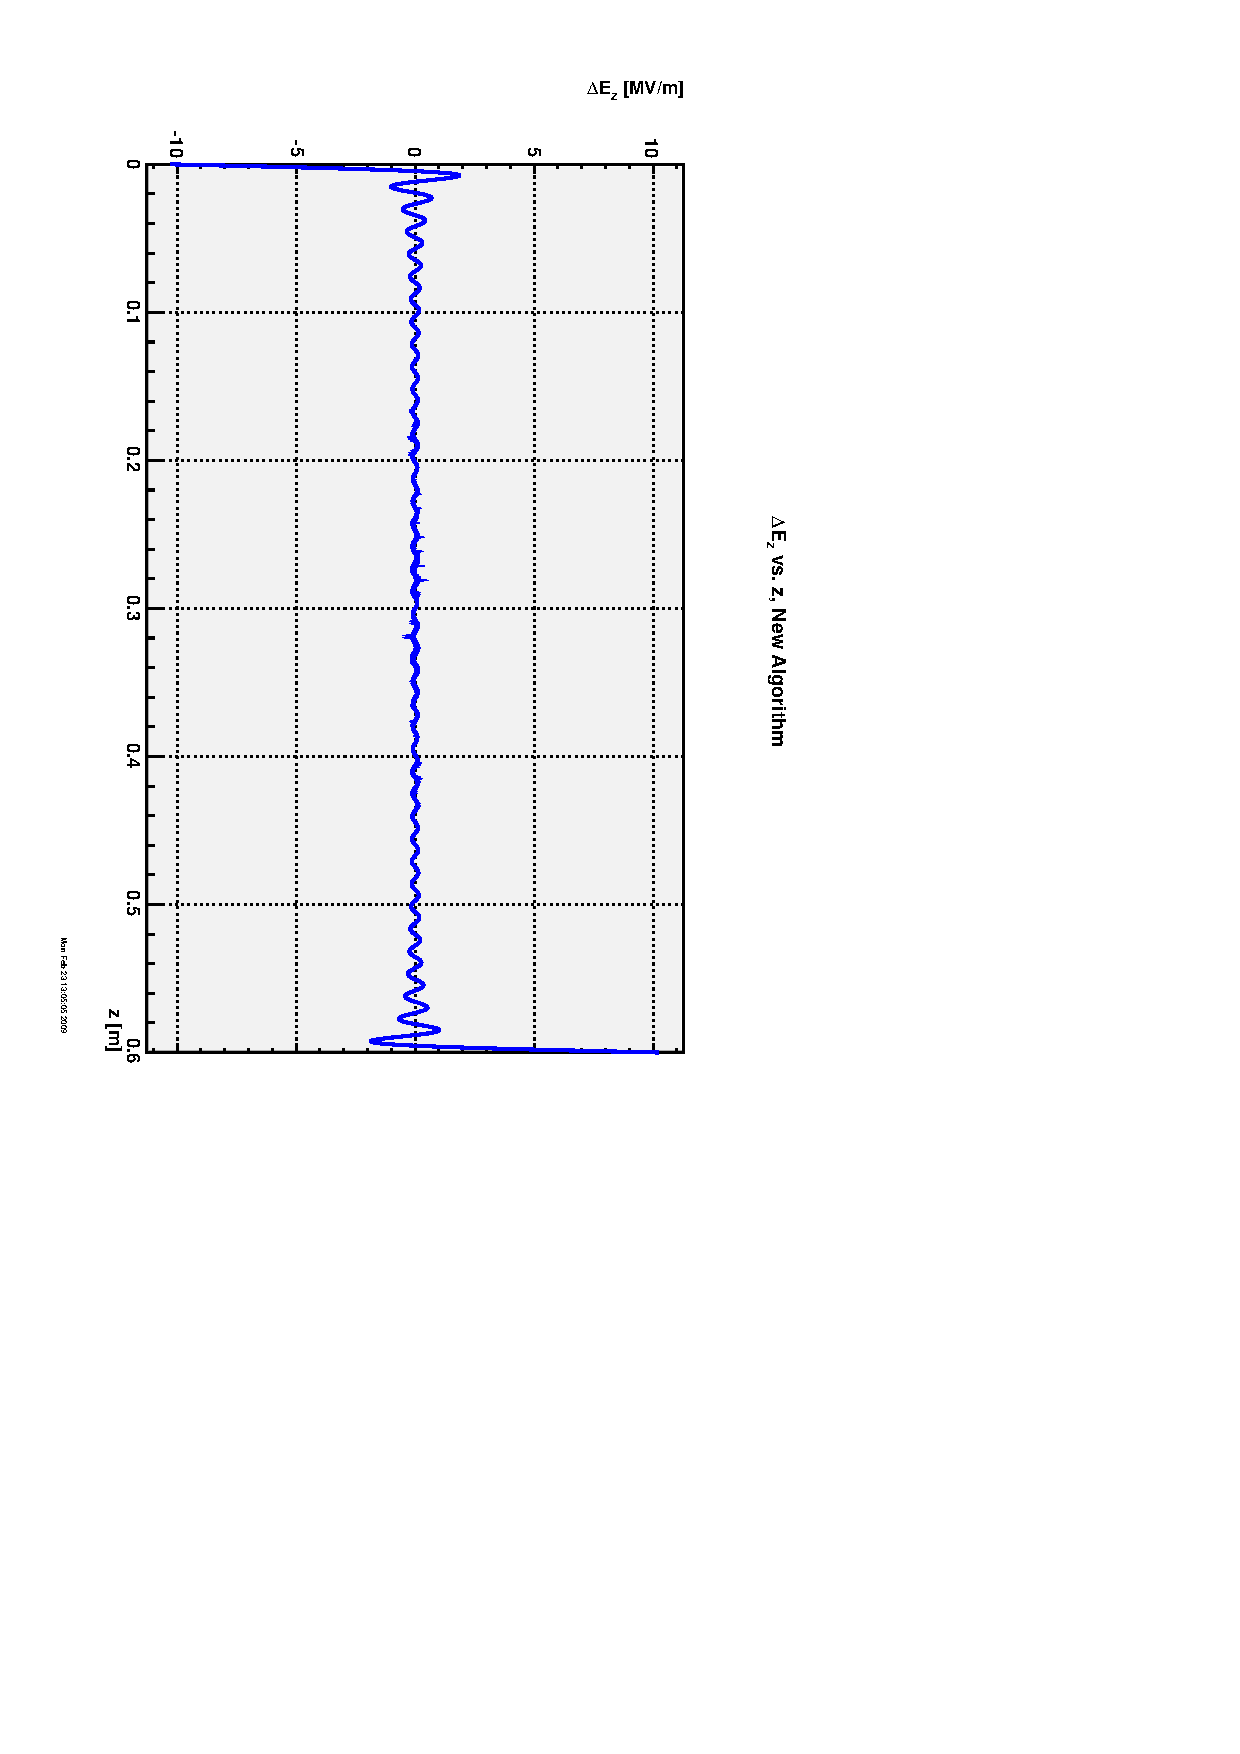
\includegraphics[scale=0.4,angle=90.0]{field-diff-new-FINLB01-MSLAC.pdf}}
  \caption{Comparison of reconstruction algorithms \eqref{E:1} and \eqref{E:2} using FINLB01-MSLAC.T7 field file.
    (The sign error in \eqref{E:2} is very apparent when we use a sin like field map.) \subref{Fi:figure-3a} Field
    from data, reconstruction using \eqref{E:1} (original) and reconstruction using \eqref{E:2} (new).
    \subref{Fi:figure-3b} Difference between original field and field reconstructed using \eqref{E:1}.
    \subref{Fi:figure-3c} Difference between original field and field reconstructed using \eqref{E:2}.}
  \label{Fi:figure-3}
\end{figure}

\end{document}